\documentclass{article}
\usepackage[utf8]{inputenc}
\usepackage{blindtext}
\usepackage{titlesec}
\usepackage{geometry}
\usepackage{listings}
\usepackage{graphicx}
\usepackage{amsfonts}
\usepackage{amssymb}
\usepackage{amsmath}
\usepackage{hyperref}
\usepackage{color}
\usepackage{float}
\usepackage{units}
\usepackage{mathtools}
\usepackage{soul}
\usepackage{enumitem}
\usepackage{siunitx}
\usepackage{multirow}
\usepackage[bottom]{footmisc}

\geometry{
 a4paper,
 total={170mm,257mm},
 left=20mm,
 top=20mm,
 }

\definecolor{codegreen}{rgb}{0.1,0.5,0.1}
\definecolor{codegray}{rgb}{0.5,0.5,0.5}
\definecolor{codepurple}{rgb}{0.58,0,0.82}
\definecolor{backcolour}{rgb}{1,1,1}
\definecolor{codemaroon}{rgb}{0.5,0,0}

\lstdefinestyle{mystyle}{
    backgroundcolor=\color{backcolour},   
    commentstyle=\color{codegreen},
    keywordstyle=\color{codemaroon},
    numberstyle=\tiny\color{codegray},
    stringstyle=\color{codepurple},
    basicstyle=\footnotesize,
    breakatwhitespace=false,         
    breaklines=true,                 
    captionpos=b,                    
    keepspaces=true,                 
    numbers=left,                    
    numbersep=5pt,                  
    showspaces=false,                
    showstringspaces=false,
    showtabs=false,                  
    tabsize=2
}

\lstset{style=mystyle}
\setlength{\parindent}{0pt}
\begin{document}

\begin{titlepage}
	\centering
	{\scshape\LARGE Imperial College London \par}
	\vspace{2cm}
	{\scshape\Large Digital Systems Design \par}
	\vspace{1cm}
	{\scshape\Large Report 2 \par}
	\vspace{2.5cm}
	{\Large\itshape Dada Oluwatomisin, CID: 0084614 \par}
	\vspace{1.0cm}
	{\Large\itshape Pranav Malhotra, CID: 00823617 \par}
	\vfill
% Bottom of the page
	{\large \today\par}
\end{titlepage}

\newpage
\tableofcontents
\newpage
\section{Task 3: Storing the Program and Data on External Memories}
In task 3, interfacing the Nios II processor with external Synchronous Dynamic Random-Access Memory (SDRAM) is introduced. The SDRAM on the DEO board provides 8MB of memory however accessing memory of-chip requires the use of a controller. The controller and the fact that the SDRAM is physically further away from the processor on the DE0 board increases the latency of instruction and data fetches.\\

The expression that is going to be evaluated in task 3 is the same as that was evaluated in task 2. The function {\tt sumVector} performs this operation and is presented in listing \ref{lst:sumVector}\\

\begin{lstlisting}[language=C, frame=single, caption={\tt sumVector}, label=lst:sumVector]
float sumVector(float x[], int M){
	int i;
	
	// initialising the sum to 0
	float sum = 0;
	
	// running through the vector sequentially and accumulating the result in sum
	for(i=0; i<M; i++)
		sum += x[i]*(1+x[i]);
		
	return sum;
}
\end{lstlisting}

\subsection{Input Vector Generation Technique}\label{sec:gen_vec}
Before the performance of the system is evaluated, it is important to note that the way floating point arithmetic is implemented has a significant impact on the precision of the result obtained. An involved discussed was presented in the previous report however an illustrative example is provided below. Consider the following function {\tt generateVectorAddition}: \\

\begin{lstlisting}[language=C, frame=single, caption={\tt generateVectorAddition}]
void generateVectorAddition(float x[N]){
	int i;
	x[0] = 0;
	
	// generating vector by accumulating result
	for(i=1; i<N; i++)
		x[i]=x[i-1]+step;
}
\end{lstlisting}


The function generates an evenly spaced vector x by initialising the first element of the vector to 0 and storing the result of successive additions. For floating point additions to be performed, the exponent of two numbers need to be equal. Thus, the first step of floating point addition involves shifting the mantissa of the smaller number\footnote{The mantissa of the smaller number is shifted to preserve the accuracy of the most significant bits.} such that both numbers have the same exponent. Following this the mantissas are added and the 23 most significant bits are kept. \textbf{This causes errors when large numbers are added to small numbers; more specifically, when the exponent of the two numbers differ by more than 23 a rounding error is incurred. The fact that the vector is generated through successive additions means that error is being accumulated.}\\

\begin{lstlisting}[language=C, frame=single, caption={\tt generateVectorMultiplication}, label=lst:generateVectorMultiplication]
void generateVectorMultiplication(float x[N]){
	int i;
	x[0]=0;
	
	// generating vector through multiplication
	for(i=1; i<N; i++)
		x[i]=i*step;
}
\end{lstlisting}

Next consider the following function {\tt generateVectorMultiplication}, presented in listing \ref{lst:generateVectorMultiplication}, that generates the vector x using single-precision floating point multiplications rather than single-precision floating point additions. The exponent of two numbers need not be equal for floating point multiplication to be performed. The two exponents are added while the two mantissas are multiplied. Moreover, any truncation error is local to each element in the vector and is not accumulated. \textbf{This implementation significantly reduces the error incurred in generating the vector x however {\tt generateVectorMultiplication} takes approximately 3.5 times longer than {\tt generateVectorAddition} to produce a vector of the same length.}\\ 
 


\begin{table}[H]
  \centering
    \begin{tabular}{|c|c|c|c|c|}
    \hline
    \multirow{2}[4]{*}{\textbf{N}} & \multirow{2}[4]{*}{\textbf{Step}} & \multirow{2}[4]{*}{\textbf{MATLAB Result}} & \textbf{{\tt generateVectorAddition}} & \textbf{{\tt generateVectorMultiplication}} \\
\cline{4-5}          &       &       & \textbf{Error from MATLAB} & \textbf{Error from MATLAB} \\
    \hline
    52    & 5     & 1144780 & 0.0000\% & 0.0000\% \\
    \hline
    511   & 0.5   & 11151936 & -0.0002\% & -0.0002\% \\
    \hline
    2551  & 0.1   & 55628996 & -0.0024\% & 0.0000\% \\
    \hline
    25501 & 0.01  & 555996390 & 0.0257\% & -0.0001\% \\
    \hline
    255001 & 0.001 & 5559670140 & -0.3756\% & 0.0007\% \\
    \hline
    \end{tabular}%
  \caption{Analysis of input vector generation techniques}
  \label{tab:generate_vector_performance}%
\end{table}%


Table \ref{tab:generate_vector_performance} summarises the results obtained. Generating the vector {\tt x} through single-precision floating point multiplications significantly reduces the error in the result. \textbf{The incredibly small percentage errors observed when a vector generated using {\tt generateVectorMultiplication} is used as an input, indicates that although evaluating the expression $\sum_{i=0}^{N}x_{i}+x_{i}^{2}$ introduces errors into the final result, the main source of the error is the inaccuracies inherent in the way the input vector is generated.}\\  

If the vectors are casted as double-precision floating point numbers, then the result of {\tt sumVector} was identical to the MATLAB result when {\tt generateVectorMultiplication} was used to generate the input vector. The percentage error when {\tt generateVectorAddition} was significantly reduced. This occurs because the truncation errors are less significant when double-precision floating point numbers are used. It is likely that MATLAB produces a linearly spaced vector using an algorithm similar to {\tt generateVectorMultiplication} since the multiplications are independent and can be implemented in parallel.\\


\textbf{This is however not the point of the exercise since our system should be able to deal with any given input vector\footnote{Optimisation of the input vector is prohibited. The input vector should be treated as a black box.}.} We did however realise a key concept in hardware design which deals with trading resources, in the form of increased memory requirements for a vector casted as a double, and the precision of our result. In generating digital systems for a specific task, the level of precision and latency requirements need to first be assessed. Once these parameters have been defined, the digital system can be optimised using a multitude of design techniques. For this specific task, it might be worth going beyond the predefined single-precision and double-precision floating point implementations and specifying custom word lengths.\\


\subsection{Latency Analysis}

The function {\tt sumVector} is evaluated and the results are presented in table \ref{tab:baseline}. The system used represents the baseline system defined in the coursework booklet. It is key to note that the time taken to evaluate {\tt sumVector} is independent of the way that the vector is generated.\\

\begin{table}[H]
  \centering
    \begin{tabular}{|c|c|c|c|c|c|}
    \hline
    \multicolumn{3}{|c|}{\multirow{2}[2]{*}{\textbf{Experimental Data: Task 3}}} & \textbf{FPGA} & \multicolumn{2}{c|}{\multirow{2}[2]{*}{\textbf{Hardware Description}}}\\
    \multicolumn{3}{|c|}{} & \textbf{Resources} & \multicolumn{2}{c|}{}\\
    \hline
    \textbf{N} & \textbf{Step} & \textbf{{\tt sumVector} (ticks)} & \multirow{6}{*}{8.57\%} & Cache Size & 2KB \\
\cline{1-3}\cline{5-6}    52    & 5     & 1     &       & On-Chip Memory & 0KB \\
\cline{1-3}\cline{5-6}    511   & 0.5   & 14    &       & Logic Elements & 3,092 / 15,408 ( 20 \% ) \\
\cline{1-3}\cline{5-6}    2551  & 0.1   & 134   &       & Memory Bits & 29,056 / 516,096 ( 6 \% ) \\
\cline{1-3}\cline{5-6}    25501 & 0.01  & 1370  &       & Embedded Multipliers & 0 / 112 ( 0 \% ) \\
\cline{1-3}\cline{5-6}    255001 & 0.001 & 13017 &       & PLLs  & 1 / 4 ( 25 \% ) \\
    \hline
    \end{tabular}%
  \caption{Latency analysis for task 3}
  \label{tab:baseline}%
\end{table}%

\subsection{Size of Application}

\textbf{The size of the NIOS II application does not change regardless of the test case used.} This is explained by understanding how the compiler uses each data segment. Below is a short description of each data segment and what they are used for.
\begin{itemize}
    \item The .data segment contains any global or static variables which have a pre-defined value and can be modified. That is any variables that are not defined within a function (and thus can be accessed from anywhere) or are defined in a function but are defined as static so they retain their value across subsequent calls.
    \item The .bss segment, also known as uninitialised data, is usually adjacent to the data segment. The BSS segment contains all global variables and static variables that are initialised to zero or do not have explicit initialisation in source code.
    \item The .rodata segment is a read-only data segment that contains static constants rather than variables.
    \item The .text segment contains the program's executable instructions. This data segment is read-only on many architectures to prevent a program from accidentally modifying instructions.\cite{wiki}  
\end{itemize}

The vector {\tt x} is initialised in the function {\tt main} and thus it is stored on the stack. The stack stores temporary variables created by each function, including {\tt main}. If memory is allocated dynamically using functions like {\tt malloc}, the variable is stored on the heap. \textbf{Both the heap and the stack do not affect the program and initialisation data size.} \\

The vector {\tt x} could have been initialised as a global vector and it would have been stored on the .data segment, however, the use of global variables should be restricted; excessive use results in increased program sizes without much benefits in terms of security of the variables. For this task, the input vector should most certainly be stored on the stack instead of on .data/.bss segment.\\ 

It should be noted that the amount of memory required on the stack increases linearly with size of the vector. Memory requirements for the three-predefined test cases are presented in table \ref{tab:vector_memory}.

\begin{table}[H]
  \centering
    \begin{tabular}{|c|c|c|}
    \hline
    \multirow{2}[4]{*}{\textbf{Size of Vector }} & \multicolumn{2}{c|}{\textbf{Memory Requirements}} \\
\cline{2-3}          & \textbf{{\tt float} (bytes)} & \textbf{{\tt double} (bytes)} \\
    \hline
    52    & 208   & 416 \\
    \hline
    2551  & 10204 & 20408 \\
    \hline
    255001 & 1020004 & 2040008 \\
    \hline
    \end{tabular}%
    \caption{Memory requirements for different test cases}
  \label{tab:vector_memory}%
\end{table}%

Table \ref{tab:vector_memory} shows the need for external memory since a vector x will not fit on the on-chip memory. \textbf{Using external memory also lifts the restrictions on the program and initialisation data size. Libraries that enable printing of floating-point numbers can now be included.}\\ 

\newpage
\subsection{Analysis of Cache Sizes}

Figure \ref{fig:latency_cache_size} shows that increasing the cache size has a positive effect on the latency of the system. There is however a plateauing effect observed.

\begin{figure}[H]
    \centering
    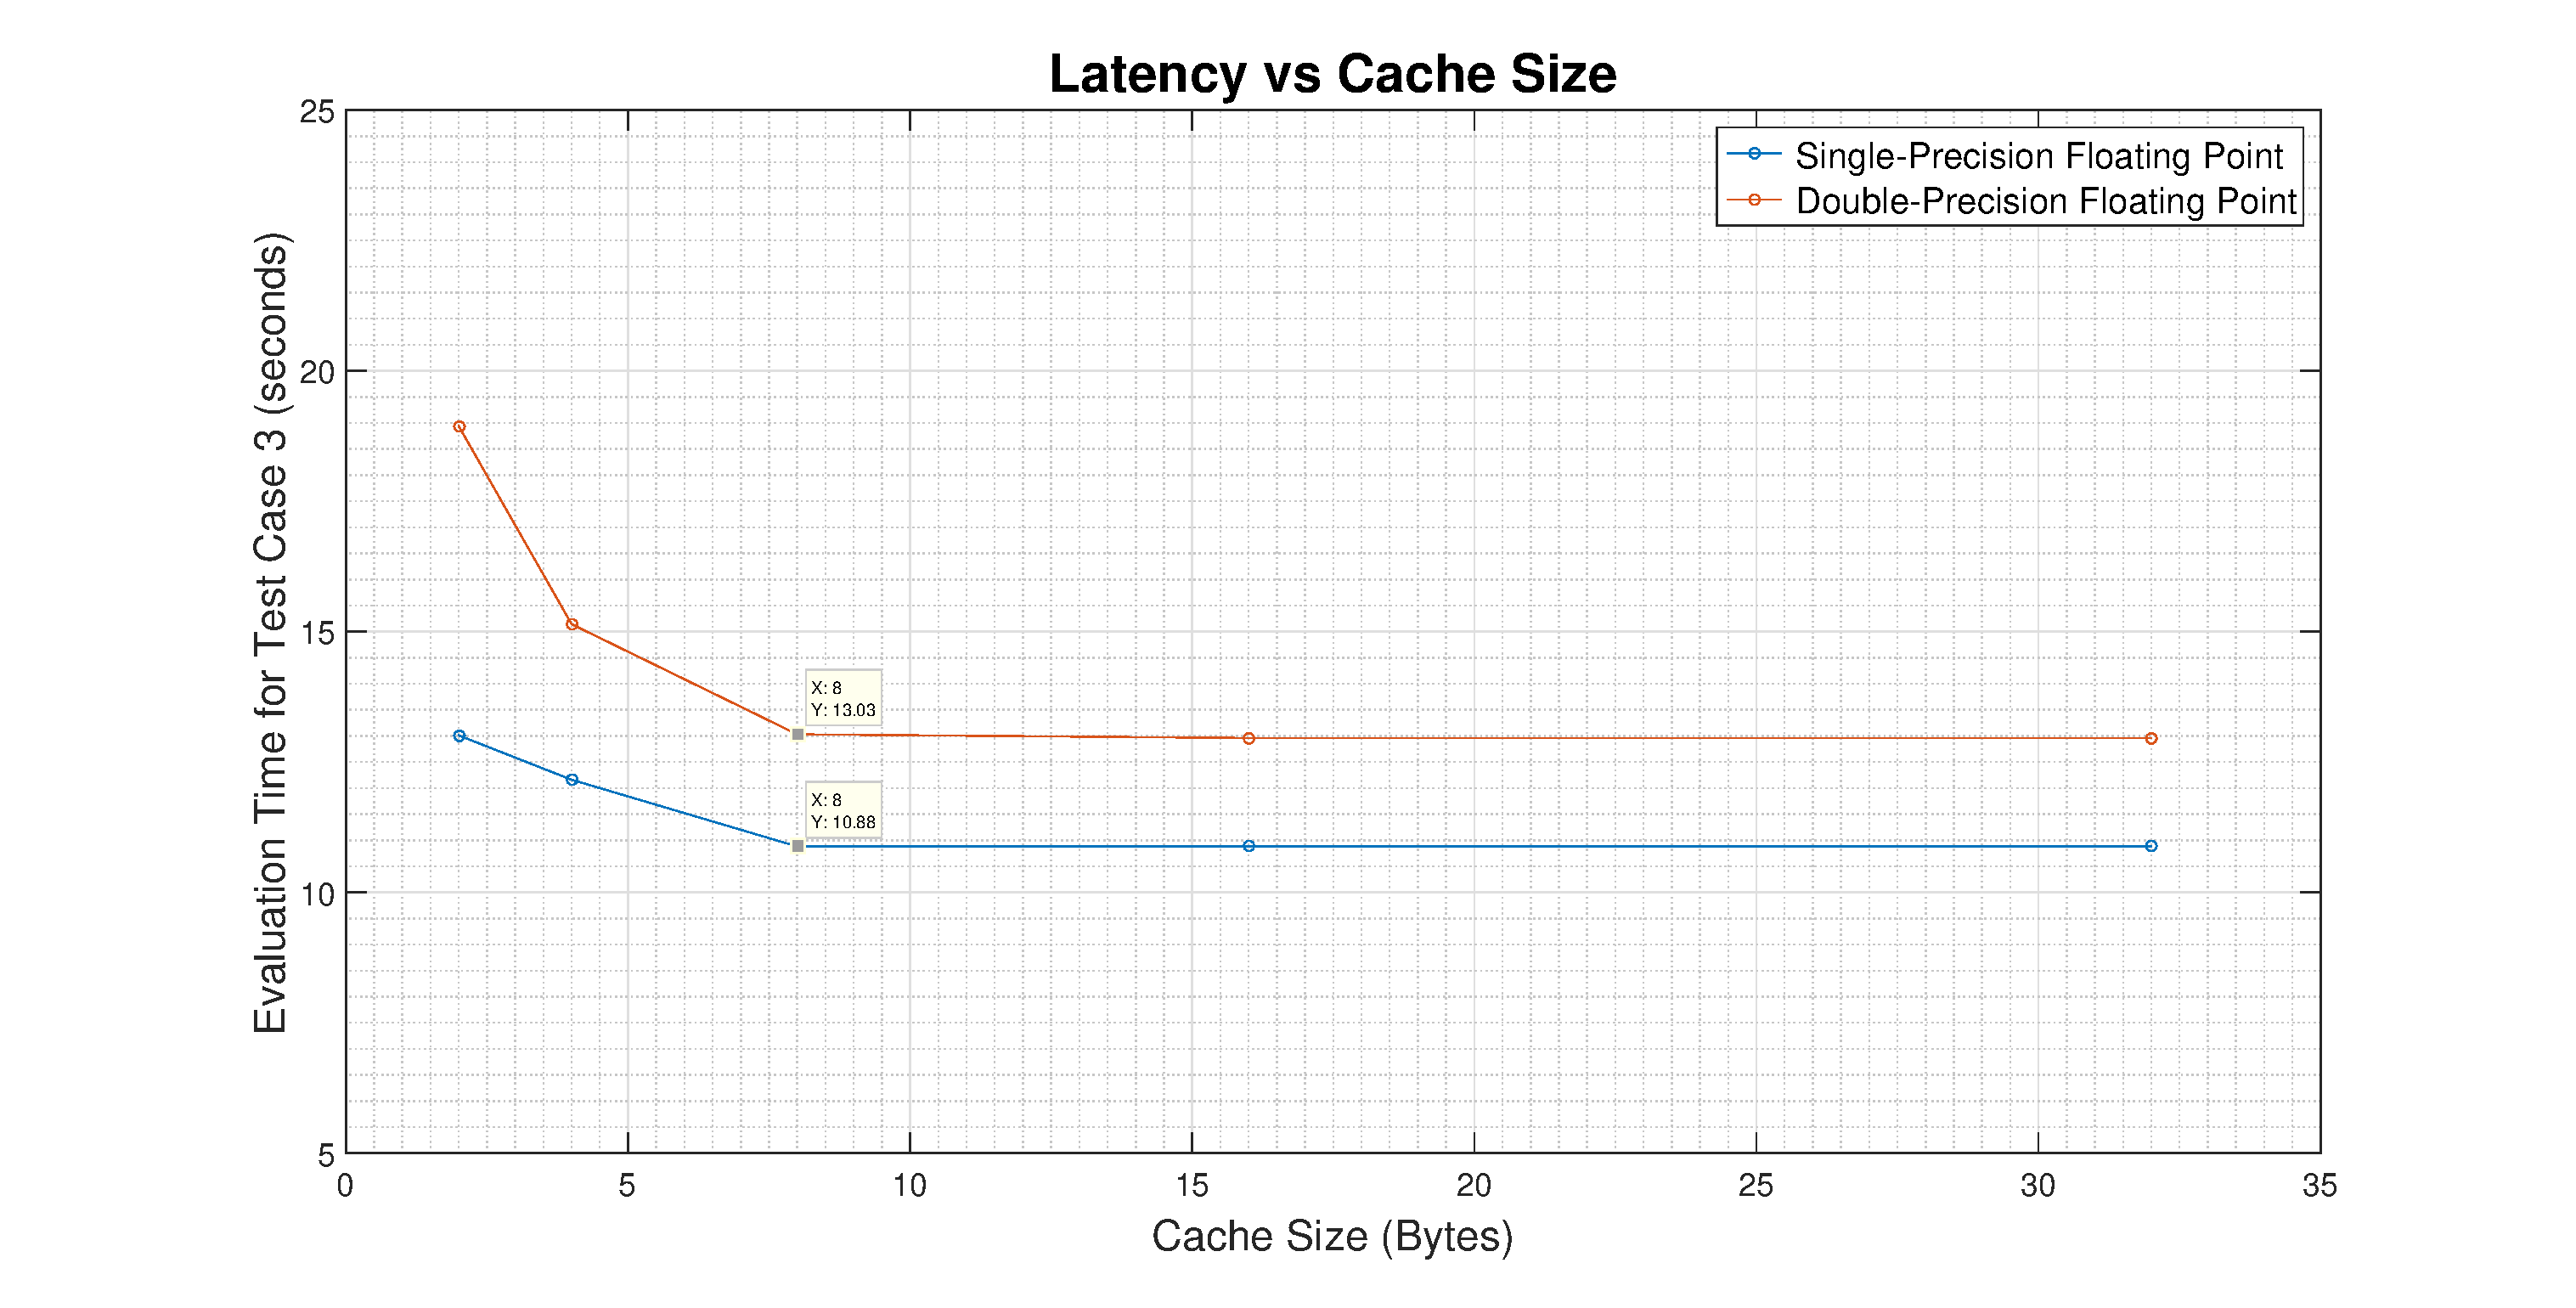
\includegraphics[width=0.99\textwidth]{graph2.eps}
    \caption{Plateauing in latency beyond 8KB of cache size}
    \label{fig:latency_cache_size}
\end{figure}

Understanding this effect requires knowledge of how caches work. Firstly, it is critical to identify the most computationally expensive part of the program, which in this case is the function {\tt sumVector}. \textbf{The {\tt for} loop runs $N$ times and to speed up the process, it would make sense to introduce a cache that is able to store all the instructions necessary to run through the loop.} Notice that having a cache that is smaller in size than the size of the for loop would not be optimal as each cycle of the loop will still require a memory fetch from the SDRAM. Putting a cache that is bigger than the size of the for loop would prevent the need for some SDRAM memory accesses at other parts of the program however this is not a good trade off as it requires more FPGA resources\footnote{This is especially true since the next available cache size is 16KB.}. \\

\textbf{The coursework requirement stipulates that the input vector should be defined as a single-precision floating point number, however, double-precision floating point numbers were nonetheless tested.} It is clear that the defining the vector as a double-precision floating point numbers increases the latency of the program. On 32-bit architectures, more instructions are required to implement addition for double-precision floating point numbers through the use of the {\tt ADC} instruction to account for the carry bit. Another source of increased latency is the fact that for each element of the vector, 8bytes of data have to be fetched instead of 4bytes in the case of a single - precision floating point number. Lastly, note that the processor does not allow the use of a data cache which can also be used to significantly reduce the latency of the program. \\

\newpage
\subsection{Final Design}

Table \ref{tab:fpga_resource_usage} provides a breakdown of the FPGA resources used for different cache sizes. 

\begin{table}[H]
  \centering
    \begin{tabular}{|c|c|c|c|}
    \hline
    \textbf{Cache Size} & \textbf{FPGA Resources } & \multicolumn{2}{c|}{\textbf{Hardware Description}} \\\hline
    \multirow{5}{*}{2KB} & \multirow{5}{*}{8.57\%} & On-Chip Memory & 0KB \\
\cline{3-4}          &       & Logic Elements & 3,092 / 15,408 ( 20 \% ) \\
\cline{3-4}          &       & Memory Bits & \textbf{29,056 / 516,096 ( 6 \% )} \\
\cline{3-4}          &       & Embedded Multipliers & 0 / 112 ( 0 \% ) \\
\cline{3-4}          &       & PLLs  & 1 / 4 ( 25 \% ) \\
    \hline
    \multirow{5}{*}{4KB} & \multirow{5}{*}{9.72\%} & On-Chip Memory & 0KB \\
\cline{3-4}          &       & Logic Elements & 3,097 / 15,408 ( 20 \% ) \\
\cline{3-4}          &       & Memory Bits & \textbf{46,720 / 516,096 ( 9 \% )} \\
\cline{3-4}          &       & Embedded Multipliers & 0 / 112 ( 0 \% ) \\
\cline{3-4}          &       & PLLs  & 1 / 4 ( 25 \% ) \\
    \hline
    \multirow{5}{*}{8KB} & \multirow{5}{*}{11.99\%} & On-Chip Memory & 0KB \\
\cline{3-4}          &       & Logic Elements & 3,097 / 15,408 ( 20 \% ) \\
\cline{3-4}          &       & Memory Bits & \textbf{81,920 / 516,096 ( 16 \% )} \\
\cline{3-4}          &       & Embedded Multipliers & 0 / 112 ( 0 \% ) \\
\cline{3-4}          &       & PLLs  & 1 / 4 ( 25 \% ) \\
    \hline
    \multirow{5}{*}{16KB} & \multirow{5}{*}{16.52\%} & On-Chip Memory & 0KB \\
\cline{3-4}          &       & Logic Elements & 3,098 / 15,408 ( 20 \% ) \\
\cline{3-4}          &       & Memory Bits & \textbf{152,064 / 516,096 ( 29 \% )} \\
\cline{3-4}          &       & Embedded Multipliers & 0 / 112 ( 0 \% ) \\
\cline{3-4}          &       & PLLs  & 1 / 4 ( 25 \% ) \\
    \hline
    \multirow{5}{*}{32KB} & \multirow{5}{*}{25.55\%} & On-Chip Memory & 0KB \\
\cline{3-4}          &       & Logic Elements & 3,098 / 15,408 ( 20 \% ) \\
\cline{3-4}          &       & Memory Bits & \textbf{291,840 / 516,096 ( 57 \% )} \\
\cline{3-4}          &       & Embedded Multipliers & 0 / 112 ( 0 \% ) \\
\cline{3-4}          &       & PLLs  & 1 / 4 ( 25 \% ) \\
    \hline
    \end{tabular}%
    \caption{FPGA resource usage overview}
    \label{tab:fpga_resource_usage}
\end{table}%


Figure \ref{fig:fpga_cache_size} shows that FPGA resources increase linearly with the size of cache used.

\begin{figure}[H]
    \centering
    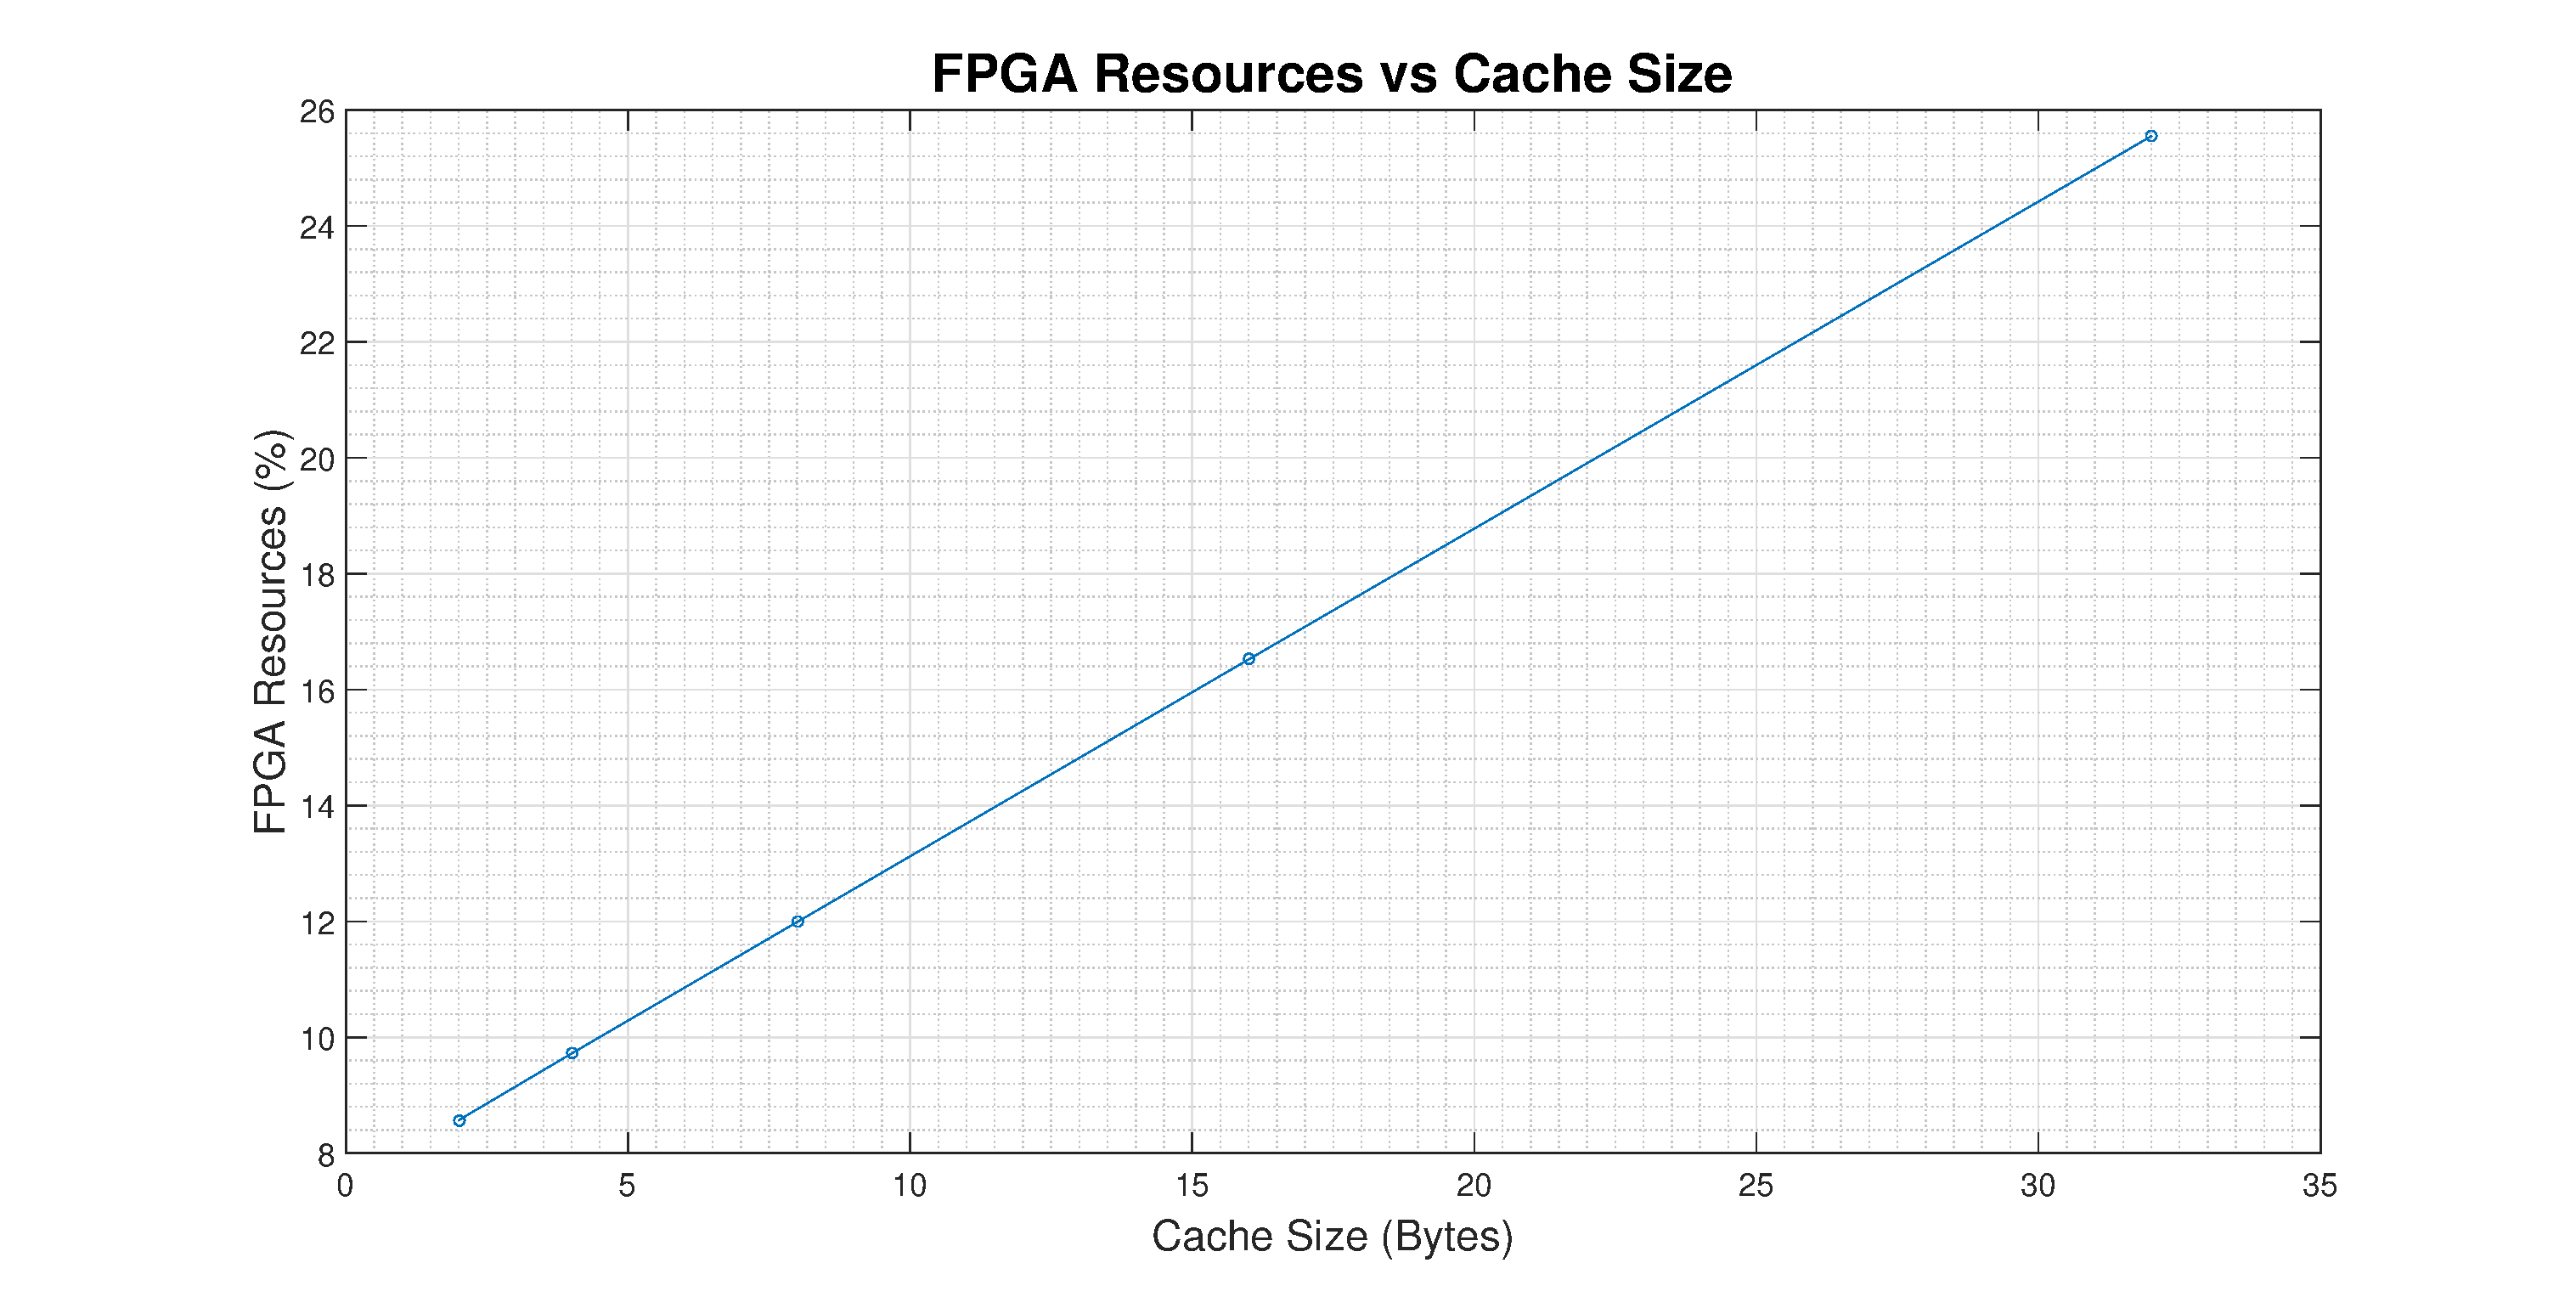
\includegraphics[width=0.9\textwidth]{graph1.eps}
    \caption{Linear increase in FPGA resources with an increase in cache size}
    \label{fig:fpga_cache_size}
\end{figure}

\textbf{Based on figure \ref{fig:latency_cache_size} and table \ref{tab:fpga_resource_usage}, the final design should make use of 8KB of cache and no on-chip memory.} This provides the best balance between the latency of the program, since increasing cache size has no significant effect on latency beyond 8KB, and resource utilisation because increasing the cache size from 4KB to 8KB only uses $2.27\%$ more resources.\\

It is obvious that the optimal cache size is in between 4KB and 8KB. The processor however only allows cache sizes that are powers of 2. Further optimisation can be done if the cache size was fully customisable. Another option to decrease the latency and speed up the program is to make use of tightly-coupled on-chip memory. 

On-chip memory is the highest throughput, lowest latency memory possible in an FPGA-based embedded system. It typically has a latency of only one clock cycle\cite{highest_throughput}. On-Chip Memory is usually used for:
\begin{itemize}
  \item Separate exception stack for use only while handling interrupts 
  \item Fast data buffers
  \item Fast sections of code
  \item Fast interrupt handler
  \item Critical loop
  \item Constant access time that is guaranteed not to have arbitration delays\cite{on-chip_memory}
\end{itemize}
\textbf{To optimise the program, the function {\tt sumVector} could be stored on the on-chip memory.} This was not implemented for these task but will be explored in further tasks. 

\subsection{Summary of Task 3}
Task 3 involved the analysing the trade-off between resources and performance. Resources are measured in terms of the logic elements, memory bits and embedded multipliers used, whereas performance is measured as the latency of the program. As discussed, the optimal point of the trade-off is identified as making use of 8KB of cache. Using a bigger cache will increase resources and power utilisation without improving performance. \textbf{In light of the fact that future tasks require a computing a more complicated function, testing for the optimal cache size will be done in task 4 as well.}

\newpage
\section{Task 4: Evaluating a More Complex Mathematical Expression}
For task 4, equation \ref{eq:1} is evaluated.

\begin{equation}
    f(x) = \sum_{i=0}^{N-1}0.5 x_{i} + x_{i}^{2}cos(floor(\frac{x_{i}}{4})-32)\label{eq:1}
\end{equation}
Listing \ref{lst:evalCosineFunc} shows the code for the function {\tt evalCosineFunc} that is used in task $4$. 

\begin{lstlisting}[language=C, frame=single, caption={\tt evalCosineFunc} function, label=lst:evalCosineFunc]
float evalCosineFunc(float x[], int M){
	int i;
	
	// initialising the sum to 0
	float sum = 0;
	
	// running through the vector sequentially and accumulating result in sum
	for(i=0; i<M; i++)
		sum+=x[i]*(0.5+x[i]*cos(floor(x[i]/4)-32));
	
	return sum;
}
\end{lstlisting}

\subsection{Cache Size Discussion}

\begin{table}[H]
  \centering
    \begin{tabular}{|c|c|c|c|c|c|}
    \hline
    \multirow{2}{*}{\textbf{N}} & \multirow{2}{*}{\textbf{Step}} & \multirow{2}[2]{*}{\textbf{Cache Size}} & \textbf{FPGA} & \textbf{{\tt sumVector}} & \textbf{Percentage Improvement}\\
          &       &       & \textbf{Resources} & \textbf{(ticks)} & \textbf{8KB Reference}\\
    \hline
    \multirow{5}{*}{255001} & \multirow{5}{*}{0.001} & 2KB   & 8.57\% & 422182 & -20.59\% \\
\cline{3-6}          &       & 4KB   & 9.72\% & 389221 & -11.18\% \\
\cline{3-6}          &       & 8KB   & 11.99\% & 350093 & 0.00\% \\
\cline{3-6}          &       & 16KB  & 16.52\% & 338152 & 3.41\% \\
\cline{3-6}          &       & 32KB  & 25.55\% & 329274 & 5.95\% \\
    \hline
    \end{tabular}%
  \caption{Analysis of optimal cache size for task 4}
  \label{tab:task4_cache_size}%
\end{table}%

Equation \ref{eq:1} was evaluated using the function {\tt evalCosineFunc} described in listing \ref{lst:evalCosineFunc} for a range of cache sizes. The results are presented in table \ref{tab:task4_cache_size} and graphed in figure \ref{fig:task4_caches}. \textbf{These results prove as further justification for the use of an 8KB cache size.} Increasing the cache size any further do not result in substantial improvements in latency but require a large amount of resources. In contrast, using 8KB of cache size represents a balanced trade-off between latency reduction and FPGA resource utilisation.\\


\begin{figure}[H]
    \centering
    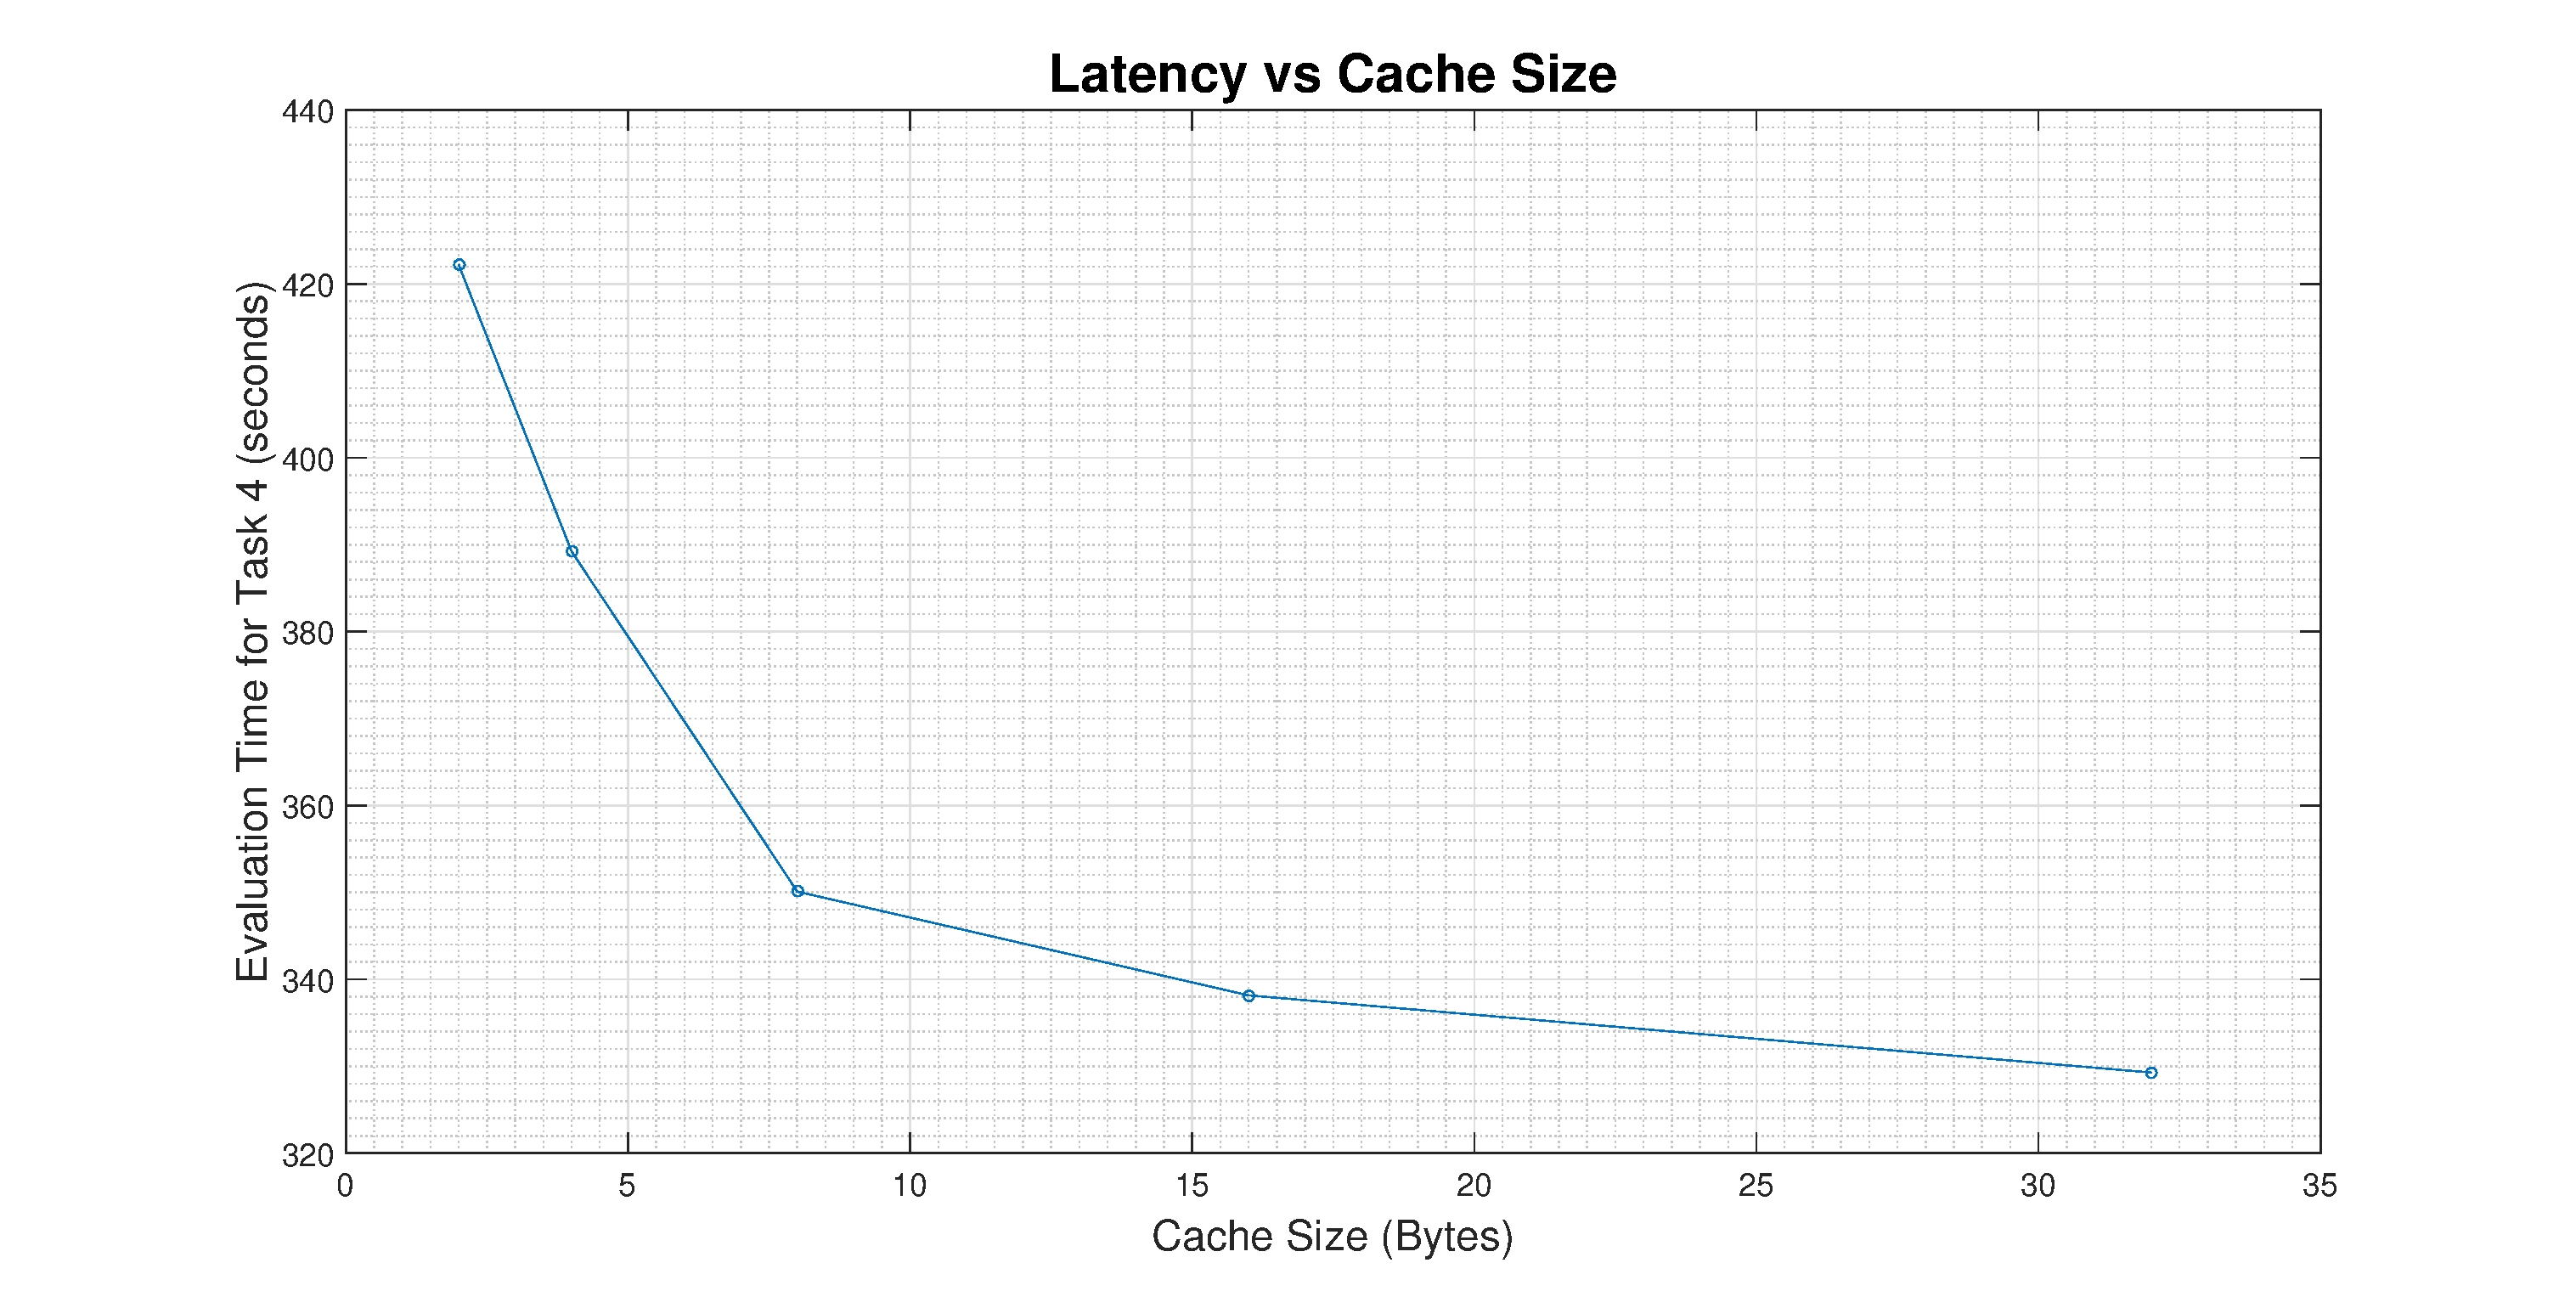
\includegraphics[width=0.9\textwidth]{graph3.eps}
    \caption{Analysis of optimal cache size for task 4}
    \label{fig:task4_caches}
\end{figure}

\textbf{However, the objective of this coursework is, given the DE0 board, to accelerate the evaluation of equation (\ref{eq:1}) as much as possible. Thus, although the balanced choice is to make use of 8KB of cache, 32KB of cache will be utilised from this point on.}

\subsection{Accuracy of Result}

As discussed as \ref{sec:gen_vec}, the accuracy of the final result is heavily dependent on the algorithm used to generate the input vector. To compare the accuracy of the results, both generation techniques discussed in section \ref{sec:gen_vec} were tested. The results are presented in table \ref{tab:task4_accuracy} and graphed in figure \ref{fig:task4_accuracy}. Note that, in accordance with coursework stipulations, both vectors are initialised as single-precision floating point integers. \textbf{The insignificant error incurred when {\tt generateVectorMultiplication} is used to generate the input vector corroborates the assertion made in section \ref{sec:gen_vec} that the main source of the error in the result is due to the inaccurate generation of the input vector.}

\begin{table}[H]
  \centering
    \begin{tabular}{|c|c|c|c|c|}
    \hline
    \multirow{2}{*}{\textbf{N}} & \multirow{2}{*}{\textbf{Step}} & \textbf{MATLAB} & \textbf{{\tt generateVectorAddition}} & \textbf{{\tt generateVectorMultiplication}} \\
\cline{4-5}          &       & \textbf{Result} & \textbf{Percentage Error} & \textbf{Percentage Error} \\
    \hline
    52    & 5     & 57880.00 & 0.0002\% & 0.0002\% \\
    \hline
    511   & 0.5   & 34026.00 & -0.0004\% & -0.0004\% \\
    \hline
    2551  & 0.1   & -68594.00 & -12.2159\% & -0.0022\% \\
    \hline
    25501 & 0.01  & -1223100.00 & -30.0492\% & 0.0024\% \\
    \hline
    255001 & 0.001 & -12768000.00 & 389.9631\% & 0.0034\% \\
    \hline
    \end{tabular}%
  \caption{Error analysis for task 4}
  \label{tab:task4_accuracy}%
\end{table}%

\begin{figure}[H]
    \centering
    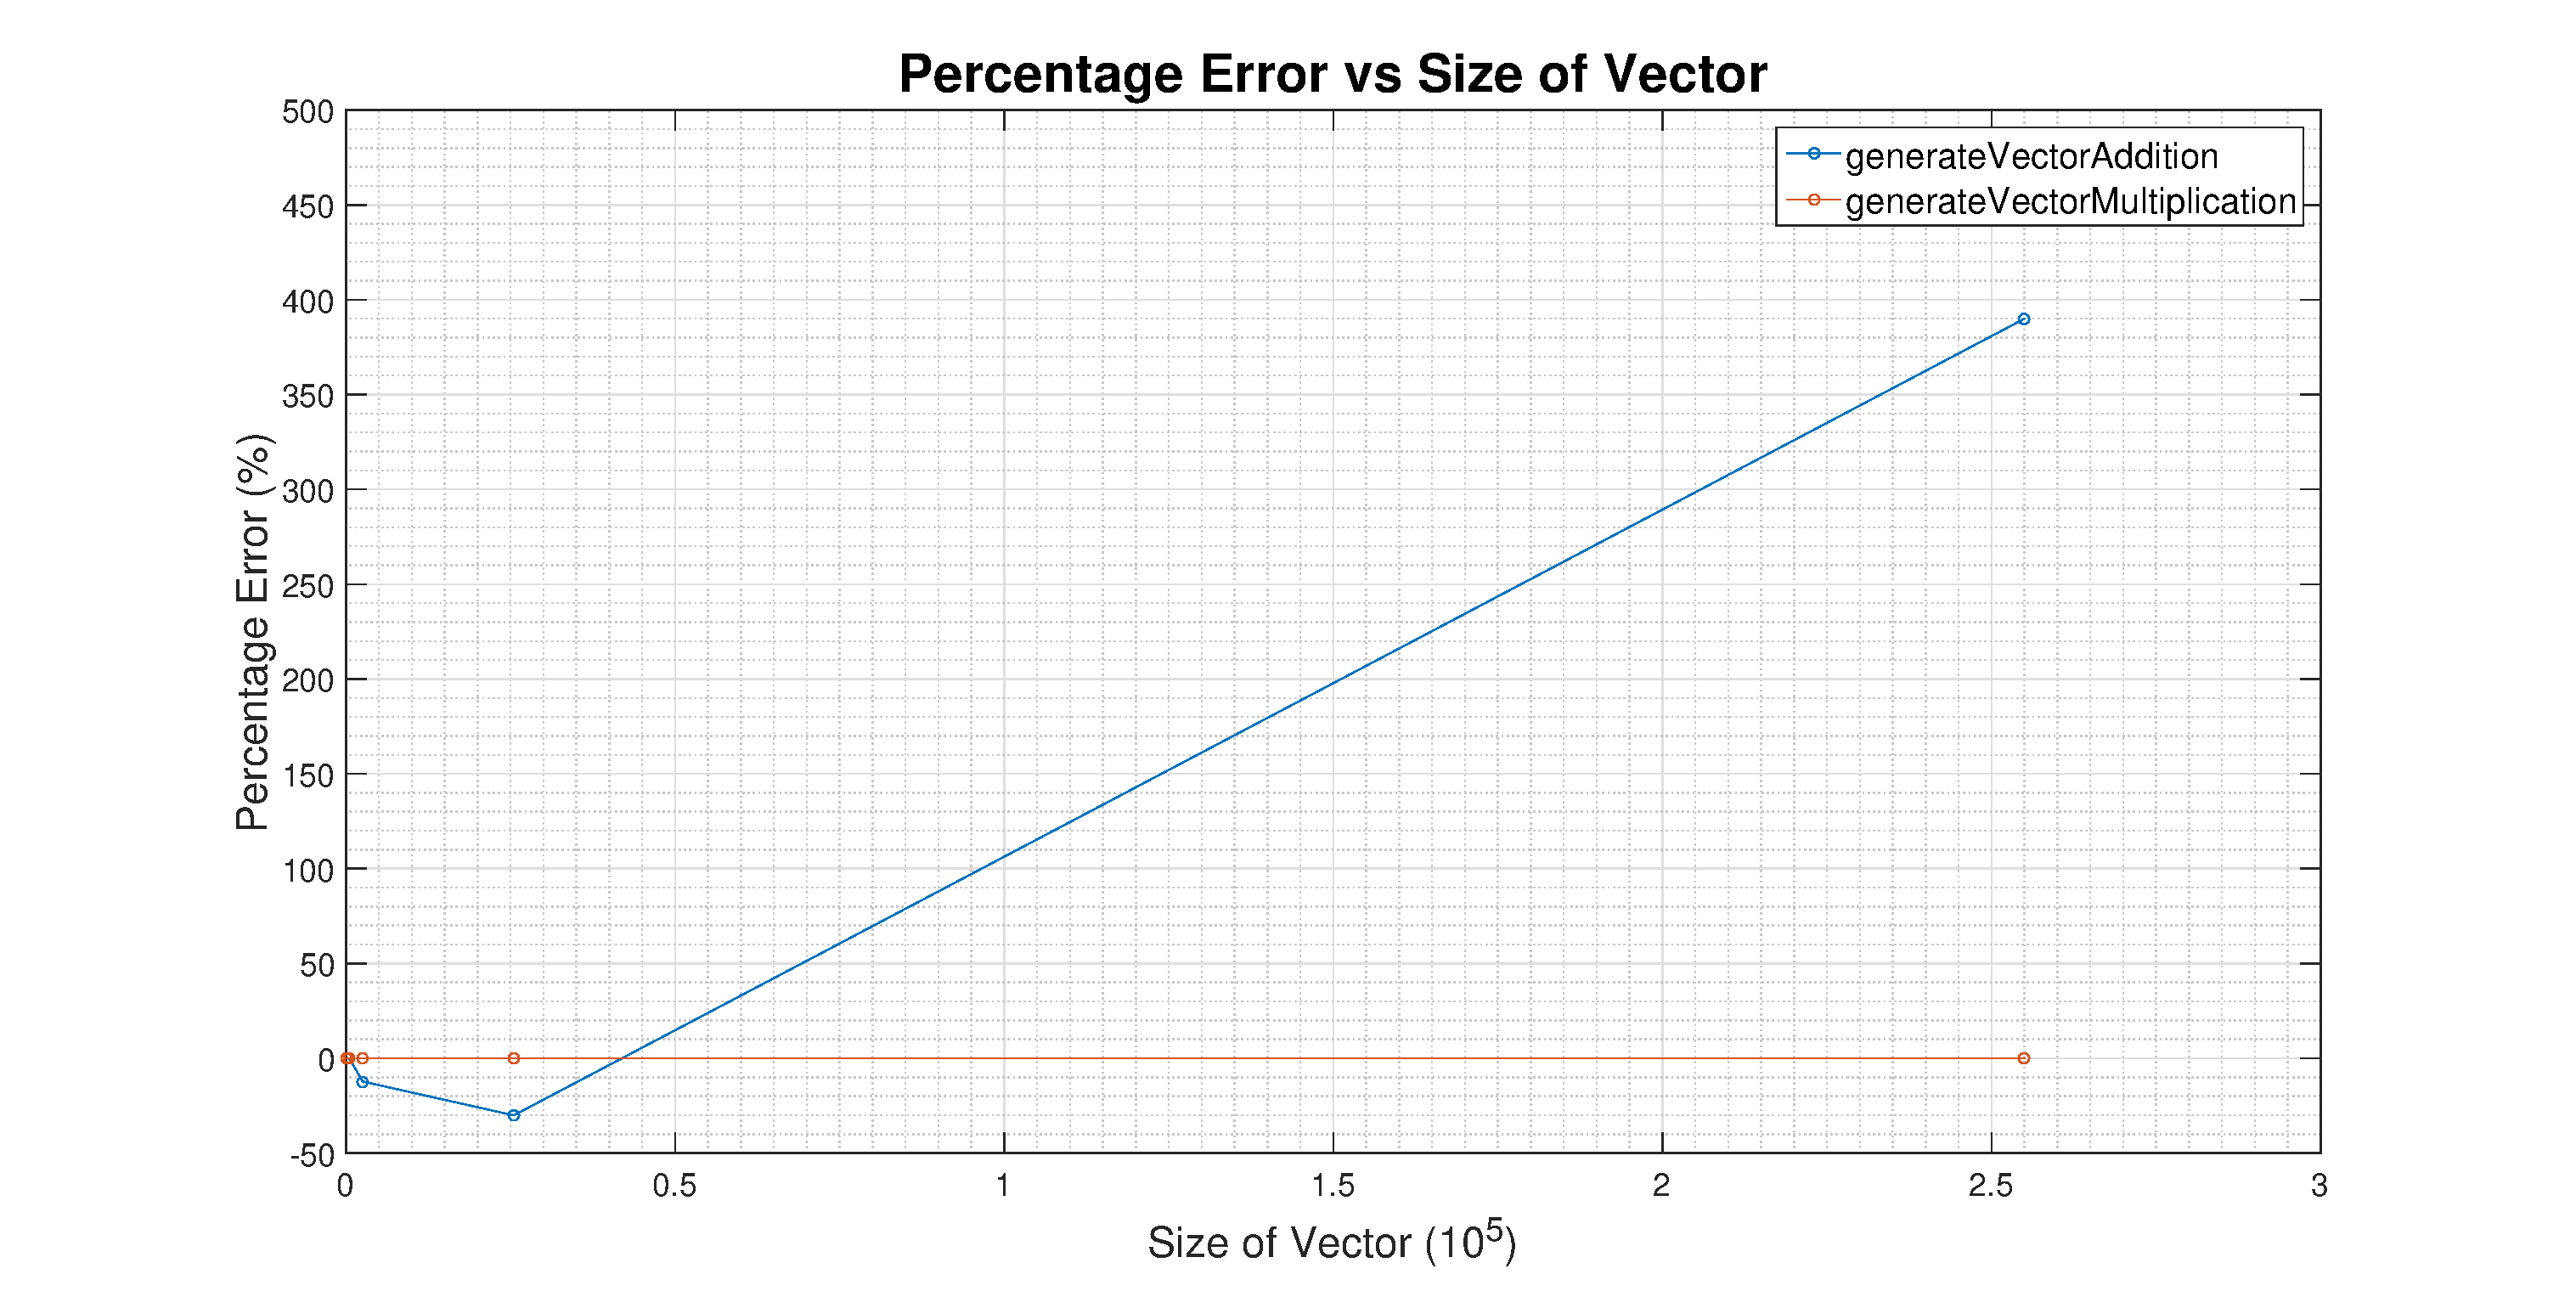
\includegraphics[width=0.9\textwidth]{graph4.eps}
    \caption{Graph of percentage error for each vector generation technique}
    \label{fig:task4_accuracy}
\end{figure}



\subsection{Implementation of Cosine using In-Built Libraries}

\textbf{The function {\tt cos} defined in the {\tt math.h} header filer is defined to take a double-precision floating point number as an input and returns a double-precision floating point number.} In the current implementation presented in listing \ref{lst:evalCosineFunc}, the cosine takes a single-precision floating point number as an input and outputs a double-precision floating point number. The rest of the expression $0.5x+x^{2}\alpha$, where $\alpha$ represents the result of the cosine is evaluated as a double-precision floating point number. Next, since the variable {\tt sum} is declared as a single-precision floating point number, an additional truncation operation is performed at every iteration. To prevent this truncation operation, the variable {\tt sum} is declared as a {\tt double}. \textbf{Since less instructions are being performed, an increase in performance is expected.} This is consistent with the results presented in table \ref{tab:double_float_task4}.

\begin{table}[H]
  \centering

    \begin{tabular}{|c|c|c|c|c|}
    \hline
    \multirow{2}[4]{*}{\textbf{N}} & \multirow{2}[4]{*}{\textbf{Step}} & \multicolumn{3}{c|}{\textbf{{\tt evalCosineFunc} (ticks)}} \\
\cline{3-5}          &       & \textbf{Variable {\tt sum}: {\tt float}} & \textbf{Variable {\tt sum}: {\tt double}} & \textbf{Percentage Improvement} \\
    \hline
    52    & 5     & 73    & 71    & 2.74\% \\
    \hline
    511   & 0.5   & 710   & 703   & 0.99\% \\
    \hline
    2551  & 0.1   & 3507  & 3479  & 0.80\% \\
    \hline
    25501 & 0.01  & 34765 & 34400 & 1.05\% \\
    \hline
    255001 & 0.001 & 350093 & 344103 & 1.71\% \\
    \hline
    \end{tabular}
  \caption{Analysis of {\tt cos} function across test cases}
  \label{tab:double_float_task4}%
\end{table}


Further proof of this trend is provided in table \ref{tab:further_proof}. 

\begin{table}[H]
  \centering
    \begin{tabular}{|c|c|c|c|c|c|}
    \hline
    \multirow{3}[4]{*}{\textbf{N}} & \multirow{3}[4]{*}{\textbf{Step}} & \multirow{3}[4]{*}{\textbf{Cache Size}} & \multicolumn{3}{c|}{\textbf{{\tt evalCosineFunc} (ticks)}} \\
\cline{4-6}          &       &       & \multirow{2}[2]{*}{\textbf{Variable {\tt sum}: {\tt float}}} & \multirow{2}[2]{*}{\textbf{Variable {\tt sum}: {\tt double}}} & \textbf{Percentage} \\
          &       &       &       &       & \textbf{Improvement} \\
    \hline
    \multirow{5}{*}{255001} & \multirow{5}{*}{0.001} & 2KB   & 422182 & 422012 & 0.04\% \\
\cline{3-6}          &       & 4KB   & 389221 & 384178 & 1.30\% \\
\cline{3-6}          &       & 8KB   & 350093 & 344103 & 1.71\% \\
\cline{3-6}          &       & 16KB  & 338152 & 332865 & 1.56\% \\
\cline{3-6}          &       & 32KB  & 329274 & 326675 & 0.79\% \\
    \hline
    \end{tabular}%
  \caption{Analysis of {\tt cos} function across cache sizes}
  \label{tab:further_proof}%
\end{table}%

\textbf{It is certainly worth defining the variable {\tt sum} as a double-precision floating point number. This design choice has no impact on FPGA resources as it is a software optimisation.} Also, this optimisation only uses an additional 4bytes of memory on the stack and thus is extremely cheap. It does however result in an average of $1.45\%$ performance improvement.\\


\subsection{Alternative Implementation of Cosine Function}
The {\tt cos} function is implemented using multiple different methods and is hardware dependent. Common techniques include:
\begin{itemize}
    \item Taylor Series Approximation
    \item COordinate Rotation DIgital Computer (CORDIC) Algorithm
    \item Chebyshev Polynomials
    \item Look-up Tables\\
\end{itemize}

Noticing the form of the input vector and the form of equation (\ref{eq:1}), a look-up table implementation might be suitable for this scenario. \textbf{The floor function will truncate the floating-point number x to an integer. This, together with the fact that the input vector is restricted to numbers between 0 and 255 makes the memory requirement for a look-up table affordable.} Only 63 values of the cosine have to be evaluated and stored. To match the performance of the {\tt cos} function evaluated using the {\tt math.h} library, the look-up table should store double-precision floating point numbers. This is an inexpensive and high performance implementation of the {\tt cos} function.\\

In the design of digital systems, it is crucial to be task-specific however allow some room for flexibility. \textbf{The above mentioned design does not work if the input vector does not stay within its pre-defined bounds.} Although, it is possible to exploit the cyclic nature of the {\tt cos} function, it would still require a large amount of memory to implement a look-up table to service an input vector with a larger range of values. \textbf{The look-up table implementation would be completely unfeasible if the {\tt floor} function was not present.}\\ 

The look-up table implementation of the cosine function was not tested; it may however be explored in the future.\\

\section{Task 5: Adding Multiplier Support}
In task 5, multiplier support is added to improve the computation power of the Nios II processor's Arithmetic Logic Unit (ALU). Up till this point, the ALU did not include dedicated hardware to perform multiplications. As such, any {\tt mult} instruction generated an exception; to handle such exceptions, the processor uses fixed point adders and shift circuitry to emulate a {\tt mult} operation. The circuit that performs shifting operations has a throughput of one bit per clock cycle and thus emulation of floating point multiplications is extremely slow. Adding multiplier support enables the ALU to perform shift and rotate operations in three to four cycles, and significantly improves the throughput of {\tt mult} operations\cite{multiplier}. \\

Multiplier support is provided through the use of either embedded multipliers or logic elements. Performance and resource usage differs for the two methods.\\

\textbf{It must be noted that both implementations only enable integer multiplications.} Floating point multiplication is more complex than integer multiplication. As mentioned in section \ref{sec:gen_vec}, to perform floating point multiplication, the exponents of the two numbers are summed and the mantissas are multiplied. Next, the result is rounded and the exponent is adjusted to bring the decimal point to the correct location. The multipliers that are included do not perform all the steps necessary for floating-point multiplication and thus the processors still needs to emulates. \textbf{Despite the need to emulate certain steps, the 23-bit mantissa is sufficiently long to still benefit from the use of hardware multipliers in its multiplication}.\\


A Nios II/s processor with embedded multipliers is capable of performing 32 by 16 bit integer multiplications\cite{multiplier}. The processor utilises four 9 by 9 bit embedded multipliers to perform this multiplication\footnote{Four 9 by 9 bit embedded multipliers can ideally perform 36 by 36 bit multiplications but are only used for performing 32 by 16 bit multiplication in the Nios II.}.Using logic elements to implement integer multiplication, the processor's ALU is only capable of performing 32 by 4 bit multiplications\cite{multiplier}.\\


\subsection{Comparison of Embedded Multiplier and Logic Elements}
Both embedded multipliers and logic elements are tested and results are presented in table \ref{tab:task5_time} and graphed in figure \ref{fig:task5_time}.\\

\begin{figure}[H]
    \centering
    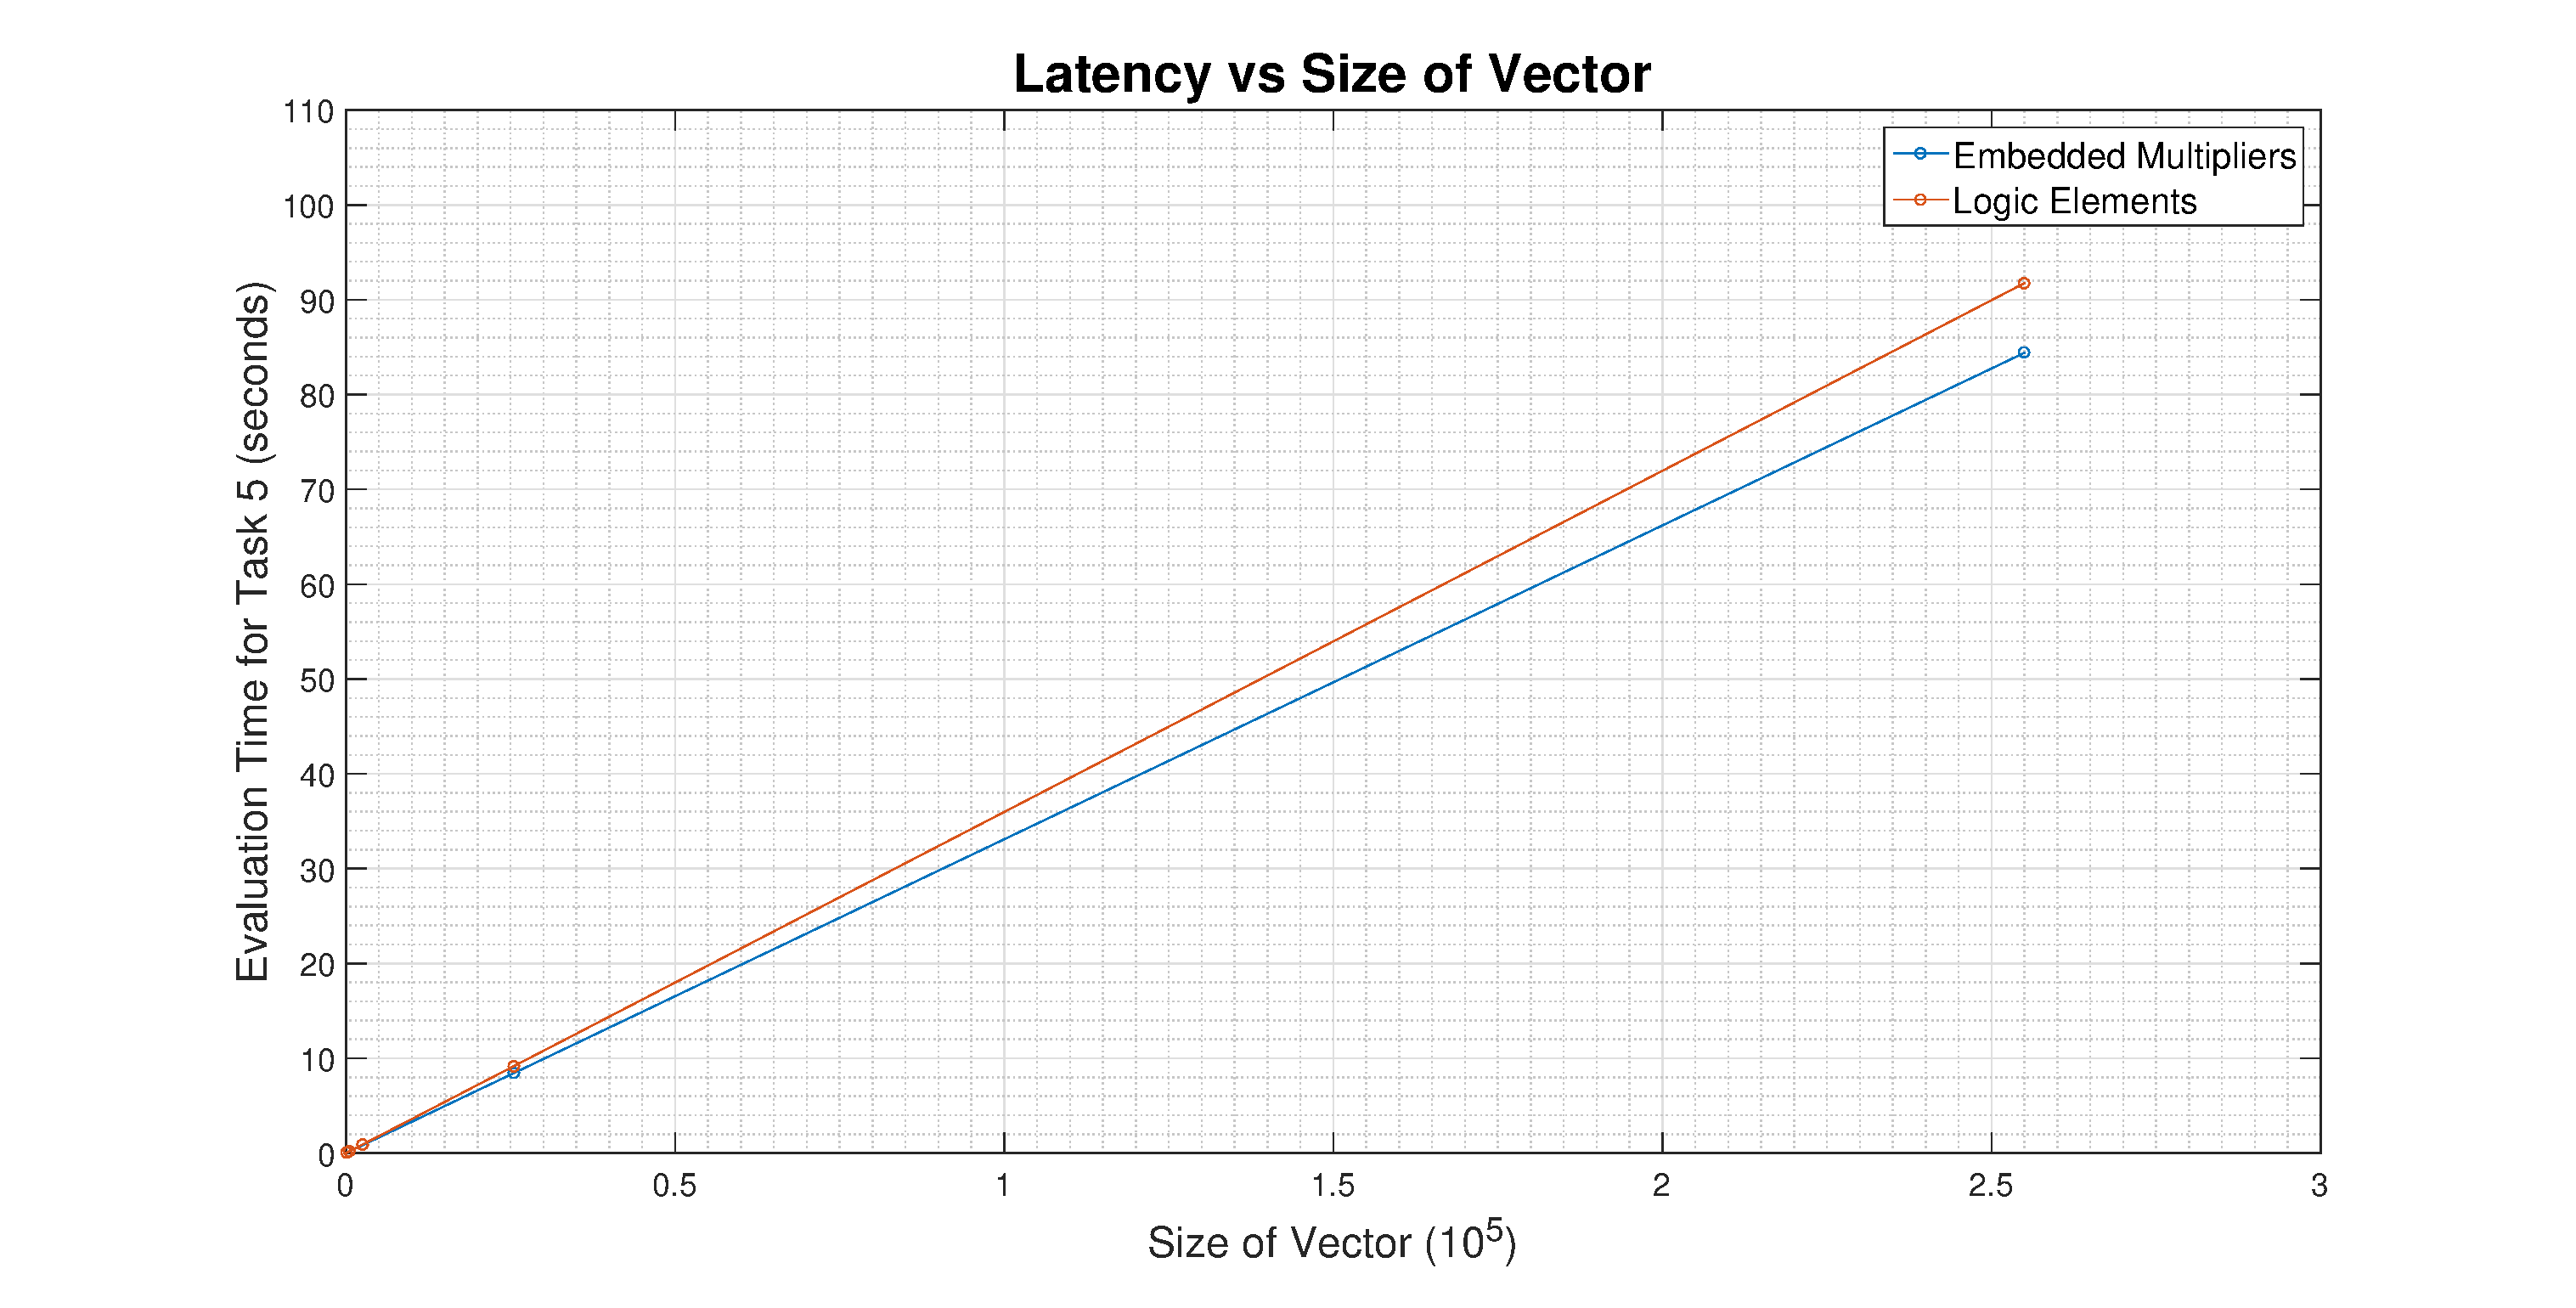
\includegraphics[width=0.9\textwidth]{graph5.eps}
    \caption{Analysis of hardware multipliers}
    \label{fig:task5_time}
\end{figure}

\begin{table}[H]
  \centering
    \begin{tabular}{|c|c|c|c|}
    \hline
    \multirow{2}[4]{*}{\textbf{N}} & \multirow{2}[4]{*}{\textbf{Step}} & \multicolumn{2}{c|}{\textbf{evalCosineFunc (ticks)}} \\
\cline{3-4}          &       & \textbf{Embedded Multipliers} & \textbf{Logic Elements} \\
    \hline
    52    & 5     & 17    & 17 \\
    \hline
    511   & 0.5   & 169   & 183 \\
    \hline
    2551  & 0.1   & 844   & 918 \\
    \hline
    25501 & 0.01  & 8440  & 9174 \\
    \hline
    255001 & 0.001 & 84401 & 91745 \\
    \hline
    \end{tabular}%
  \caption{Analysis of hardware multipliers}
  \label{tab:task5_time}%
\end{table}%



The amount of FPGA resources that each of these two methods utilise is different. The amount of resources used are detailed in table \ref{tab:task5_resources}.\\

\begin{table}[H]
  \centering
    \begin{tabular}{|c|c|c|}
    \hline
    \multicolumn{3}{|c|}{\textbf{Embedded Multipliers}} \\
    \hline
    \multicolumn{2}{|c|}{\textbf{Hardware Description}} & \textbf{FPGA Resources} \\
    \hline
    Cache Size & 32KB  & \multirow{6}{*}{27.11\%} \\
\cline{1-2}    On-Chip Memory & 0KB   &  \\
\cline{1-2}    Logic Elements & 3,270 / 15,408 ( 21 \% ) &  \\
\cline{1-2}    Memory Bits & 291,840 / 516,096 ( 57 \% ) &  \\
\cline{1-2}    PLLs  & 1 / 4 ( 25 \% ) &  \\
\cline{1-2}    Embedded Multiplier 9-bit elements & 4 / 112 ( 4 \% ) &  \\
    \hline
    \multicolumn{3}{|c|}{\textbf{Logic Elements}} \\
    \hline
    \multicolumn{2}{|c|}{\textbf{Hardware Description}} & \textbf{FPGA Resources} \\
    \hline
    Cache Size & 32KB  & \multirow{6}{*}{26.18\%} \\
\cline{1-2}    On-Chip Memory & 0KB   &  \\
\cline{1-2}    Logic Elements & 3,389 / 15,408 ( 22 \% ) &  \\
\cline{1-2}    Memory Bits & 291,840 / 516,096 ( 57 \% ) &  \\
\cline{1-2}    PLLs  & 1 / 4 ( 25 \% ) &  \\
\cline{1-2}    Embedded Multiplier 9-bit elements & 0/ 112 (0 \% ) &  \\
    \hline
    \end{tabular}%
\textbf{}
  \label{tab:task5_resources}%
\end{table}%

\subsection{Summary of Task 5}
Embedded multipliers utilise $0.93\%$ more resources than logic elements however they offer the best performance. Using embedded multipliers, 32 by 16 bit multiplications can be performed in 5 clock cycles and shifts/rotates are executed in 3 cycles.  Using logic elements to implement multiples, 11 clock cycles are required to perform a 32 by 4 bit multiplications and shifts/rotates are executed in 4 clock cycles\cite{multiplier}. \textbf{Embedded multipliers are the optimal choice to provide dedicated hardware for multiplication as they improved performance by a greater amount than logic elements.}

\section{Conclusion}
Task 3, 4 and 5 have revealed multiple challenges and design choices faced by digital systems designers. Firstly, the shortcomings of number representations were explored. Secondly, the trade-off between precision, latency and memory usage were considered. Lastly, by significantly increasing utilisation of resources, in the form of a bigger cache and embedded multipliers, a marked reduction in latency was observed. 


\newpage
\begin{thebibliography}{99}
\bibitem{wiki} Data Segment. (n.d.). Retrieved January 26, 2016, from \url{https://en.wikipedia.org/wiki/Data_segment}.
\bibitem{highest_throughput} Corporation, A. (2010). Memory System Design. Retrieved January 26, 2016, from \url{https://www.altera.com/content/dam/altera-www/global/en_US/pdfs/literature/hb/nios2/edh_ed51008.pdf}.
\bibitem{on-chip_memory} Corporation, A. (2011). . Using Tightly Coupled Memory with the Nios II Processor. Retrieved January 26, 2016, from \url{https://www.altera.com/content/dam/altera-www/global/en_US/pdfs/literature/tt/tt_nios2_tightly_coupled_memory_tutorial.pdf}.
\bibitem{multiplier}Corporation, A. (n.d.). Embedded Multipliers in the Cyclone III Device Family. Retrieved February 13, 2016, from \url{https://www.altera.com/en_US/pdfs/literature/hb/cyc3/cyc3_ciii51005.pdf}

\end{thebibliography}

\end{document}